
\subsubsection{Сущности}

\begin{enumerate}
  \item \textbf{Пользователь}: 
        идентификатор в HR системе, 
        ФИО.

  \item \textbf{Менеджер}: 
        является Пользователем, 
        связывается с заявками на перемещение,
        поставку и изъятие.

  \item \textbf{Администратор}:
        является Пользователем,
        управляет хранилищем,
        связывается с запросами на перемещение,
        поставку и изъятие,
        связывается с фактами поставки и изъятия.

  \item \textbf{Перевозчик}:
        note: отдельные таблицы для каждого,
        название перевозчика.

  \item \textbf{Заказчик}
        note: отдельные таблицы для каждого,
        название заказчика.

  \item \textbf{Хранилище}:
        содержит ячейки для хранения предметов,
        связано с Администратором,
        связано с операциями с ним.

  \item \textbf{Ячейка хранения}:
        хранилище в котором находится,
        хранит предметы одного типа,
        имеет тип хранимого предмета,
        имеет вместимость хранимых предметов.

  \item \textbf{Тип предмета}:
        имеет название,
        срок годности,
        единицы измерения 
        и прочую информацию.

  \item \textbf{INLINE Группа предметов}:
        идентификатор,
        тип предмета,
        количество > 0,
        дата изготовления,
        может быть заказ.

  \item \textbf{Перемещение}:
        идентификатор поездки у перевозчика,
        идентификатор перевозчика,
        дата отправления,
        дата прибытия,
        группы предметов,
        заявка на отправление,
        заявка на прибытие.

  \item \textbf{Заказ}
        заказчик,
        дата создания,
        дедлайн,
        связывается с перемещениями,
        связывается с изъятиями,
        мб связывается с поставками.

  \item \textbf{Поставка}
        поставщик,
        заявка на поставку,
        группы предметов.

  \item \textbf{INLINE Заявка в хранилище}
        хранилище,
        инициатор Менеджер,
        обработчик Администратор,
        принято в обработку,
        выполнено,
        дополнительная информация.

  \item \textbf{Изъятие}
        заказчик,
        заказ,
        заявка на изъятие,
        группы предметов.
  
  \item \textbf{Бронирование}
        заявка на бронирование,
        группа предметов,
        дата начала,
        дата снятия.

\end{enumerate}

\newpage

\subsubsection{Высокоуровневая ER-диаграмма}

\begin{figure}[h!]
      \centering
      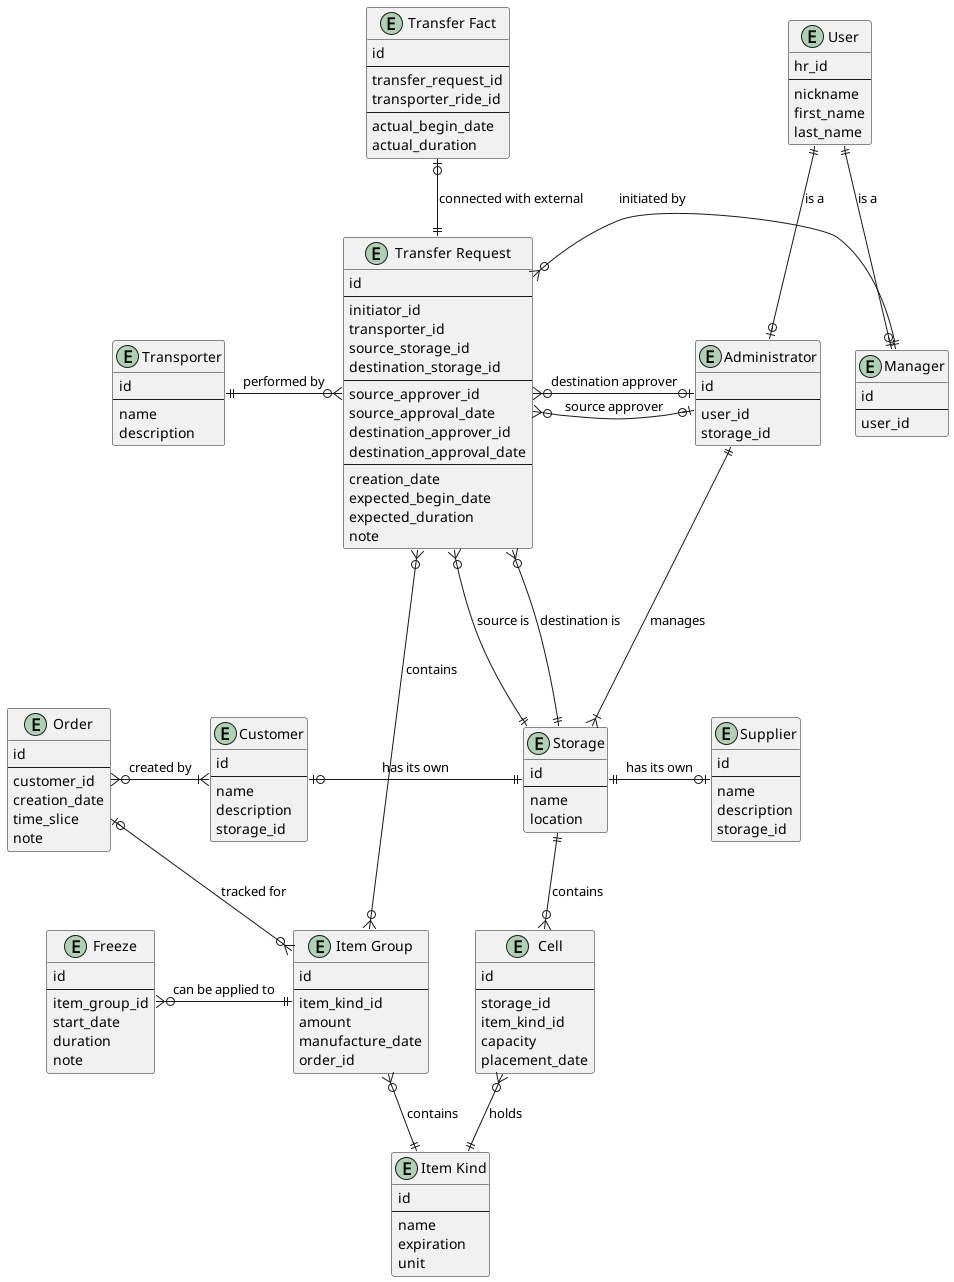
\includegraphics[width=12cm]{../../doc/spec/figure/er/high-level/Storage Net high-level ER Diagram.png}
      \caption{High-Level ER-Diagram}
\end{figure}

\newpage

\subsubsection{Низкоуровневая ER-диаграмма}

\begin{figure}[h!]
      \centering
      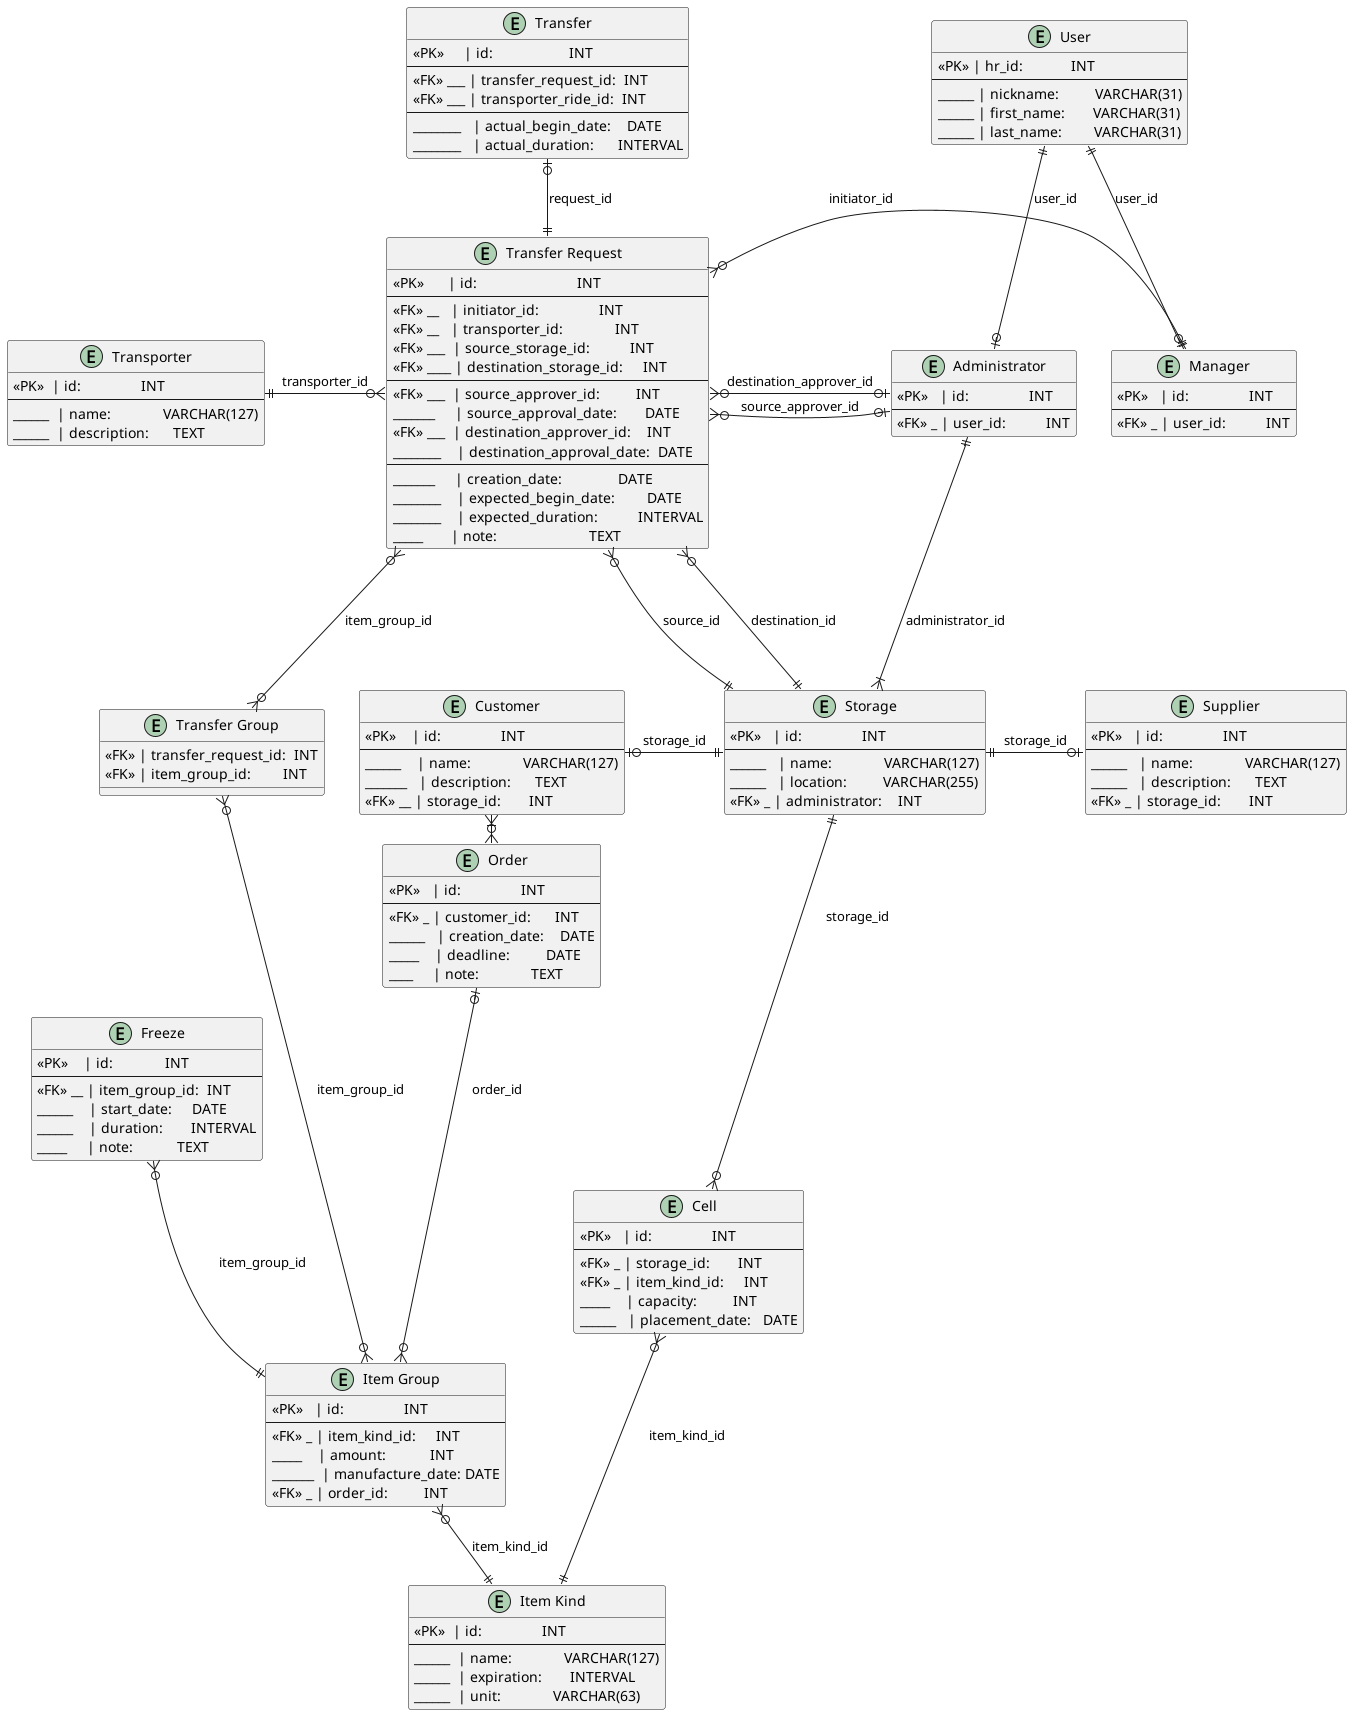
\includegraphics[width=12cm]{../../doc/spec/figure/er/low-level/Storage Net low-level ER Diagram.png}
      \caption{Low-Level ER-Diagram}
\end{figure}

\newpage